\documentclass[../main.tex]{subfiles}
\graphicspath{{\subfix{../images/}}}

\begin{document}

\begin{newrequirements}
    \textbf{Note that this section is a substantial 
    portion of the grade for your final 
    report and will require a significant 
    amount of effort.}

    \begin{todolist}
    \item describe in detail the tests you have 
        conducted to verify that your prototype 
        satisfies the desired functional 
        requirements while meeting the design 
        constraints. For example, if you used 
        Use Cases to describe your non-
        functional requirements, then for each 
        use case you should write a test case, 
        run it and report the testing results
        (the key test cases can be added as an 
        Appendix). Functional testing will 
        allow you to find defects then fix them 
        and also identify possible 
        improvements.  You need to have a 
        comprehensive set of tests that 
        verifies correct functionality of every 
        component of your system. 

    \item verify and provide evidence through 
        testing that your solution solved the 
        stated problem and satisfied the 
        requirement specifications and design 
        constraints, documented in Section 3.2 
        of the interim report. If not, explain 
        what is lacking and identify possible 
        improvements 

    \item This section must present sufficient 
        evidence and clear discussion that your 
        design and prototype met/did-not-meet 
        all of the identified technical and 
        practical constraints documented in 
        Section 3.2. You may use a summary 
        table to elaborate these points. The 
        table columns could contain: 

    \begin{todolist}
    \item Brief description of the constraints 

    \item Explanation of the testing steps taken 
        to evaluate if the constraint was met 
        or not. 

    \item Measurements data that prove your 
        system met/did-not-meet the constraint. 
        Also compare measured data against 
        expected values, then include a \%error 
        as (actual – expected)/expected*100\%, 
        and use only three digits of precision. 
        In case a constraint is not met, then 
        explain the reason for that. 
    \end{todolist}

    \item For further details and examples refer 
        to the document titled ‘Examples of how 
        to address and verify some of the 
        design constraints’ posted on the 
        Senior Projects website. 
         
    \item Describe in detail the tests performed 
        on the individual subsystems of your 
        project.  Discuss how you tested each 
        subsystem and what the results of each 
        test were. 

    \item In addition, do not forget to include: 

    \begin{todolist}
    \item If you have a GUI of some type, you 
        need a screen shot of it. 

    \item If you have a physical display of some 
        type (LEDs, LCDs, etc.), you need a 
        photograph of the display showing 
        typical operation. 

    \item For any interfaces of your hardware 
        components – USB, I2C, SPI, RS232, 
        parallel interfaces, or A/D inputs – 
        you may show oscilloscope pictures that 
        demonstrate a sample data transfer of 
        this interface and the typical 
        voltage/frequency ranges. 
    \end{todolist}

    \item You should present the test results, 
        with appropriate level of details in 
        addition to accuracy and completeness, 
        using tables, graphs, diagrams, screen 
        shots etc. Additionally, discuss these 
        results and explain whether the 
        prototype has achieved the 
        requirements. If not state what is 
        lacking or still need improvement then 
        explain the reason for that. There will 
        probably be multiple subsections under 
        this section to describe each system 
        test and its result. 

    \end{todolist}
\end{newrequirements}

\begin{table}[H]
    \centering
    \caption{Summary of the prototype testing}
    \label{tab:testing-summary}
    \begin{tabularx}{\textwidth}{ l X l l l }
        \toprule
        \textit{Constraint} 
            & \textit{Testing procedure} 
                & \textit{Result}
        & \textit{Measurement data} 
            & \textit{Error (\%)} \\

        \midrule
        
        
        ??    & ?? 
        & Met
            & ??
        & 5 \\

        \bottomrule		
    \end{tabularx}
\end{table}

%% Each subsection corresponds to a test.
%% Title the subsection based on the functional requirement OR
%% the design constraint being tested.

% HARDWARE
\subsection{Connecting to the drone}

We have connected the
Raspberry Pi to the drone using built-in WiFi
to allow Raspberry to send/receive control and status 
instructions to the drone. 
For connecting Raspberry Pi and the laptop, 
we used the external WiFi adapter and turned 
on the hotspot feature to create an access point,
and this made the process so convenient because 
once the Raspberry Pi boots up, it turns on the 
access point, and the user can connect to it 
easily and execute scripts using \textsc{ssh} 
protocol or open the web app user interface 
at www.aireye.com:8000. We executed the takeoff 
and move forward scripts and it worked successfully, so
we confirm that we can connect to the drone and can control it.

\subsection{Command-Control system maximum distance}



\subsection{Flying duration & Batteries}

\lipsum[1]

\subsection{Response time}

We have done another experiment regarding the response time 
of the drone after sending a command to it from the Raspberry Pi. 
Calculating the response time was by starting a timer when 
sending the command and stopping it when the 
state of the drone changes. 
The experiment was done on simulation using Sphinx,
then we have moved to the real world using the \anafi drone.
From \cref{tab:respone-time}, 
we can see that all the results are less than \SI{1}{second}
which satisfied our response time constraint.
Another thing we can conclude from the table is that 
the response time of the real world is less than 
the simulation, and this is predictable since the simulation
depends on the \textsc{gpu} power and processing time. 

\begin{table}[tbp]
	\centering
	\caption{The average response time of the drone after sending a control command.}
	\label{tab:respone-time}
	\begin{tabularx}{0.7\textwidth}{ X c c }
		\toprule
		\textit{} & \textit{Simulation} & \textit{Real-world}\\ \midrule
		Motor ramping for takeoff (seconds)  & 0.3506 & 0.0323     \\
		Move while flying (seconds) & 0.7441  & 0.1511   \\
		\bottomrule
	\end{tabularx}
\end{table} 

\subsection{Payload}

As shown in \cref{fig:payload}
we attached \SI{190}{grams} of Raspberry Pi and Arduino boards
to see the effect on the performance and flight and
battery drain percentage. 
The drone has taken off  successfully, 
and the flight was normal but, we faced an expected 
battery drain that went from 
\SI{100}{\percent} to \SI{90}{\percent} in 
\SI{1.5}{minutes}.This is because the propeller motors will try to push 
their limits to take off the drone, which will consume more energy.
After adding payload to the drone at \SI{200}{grams}, the drone couldn't
takeoff and we now know the limit, which will be considered in the 
design constraints.


\begin{figure}[bp]
	\centering
	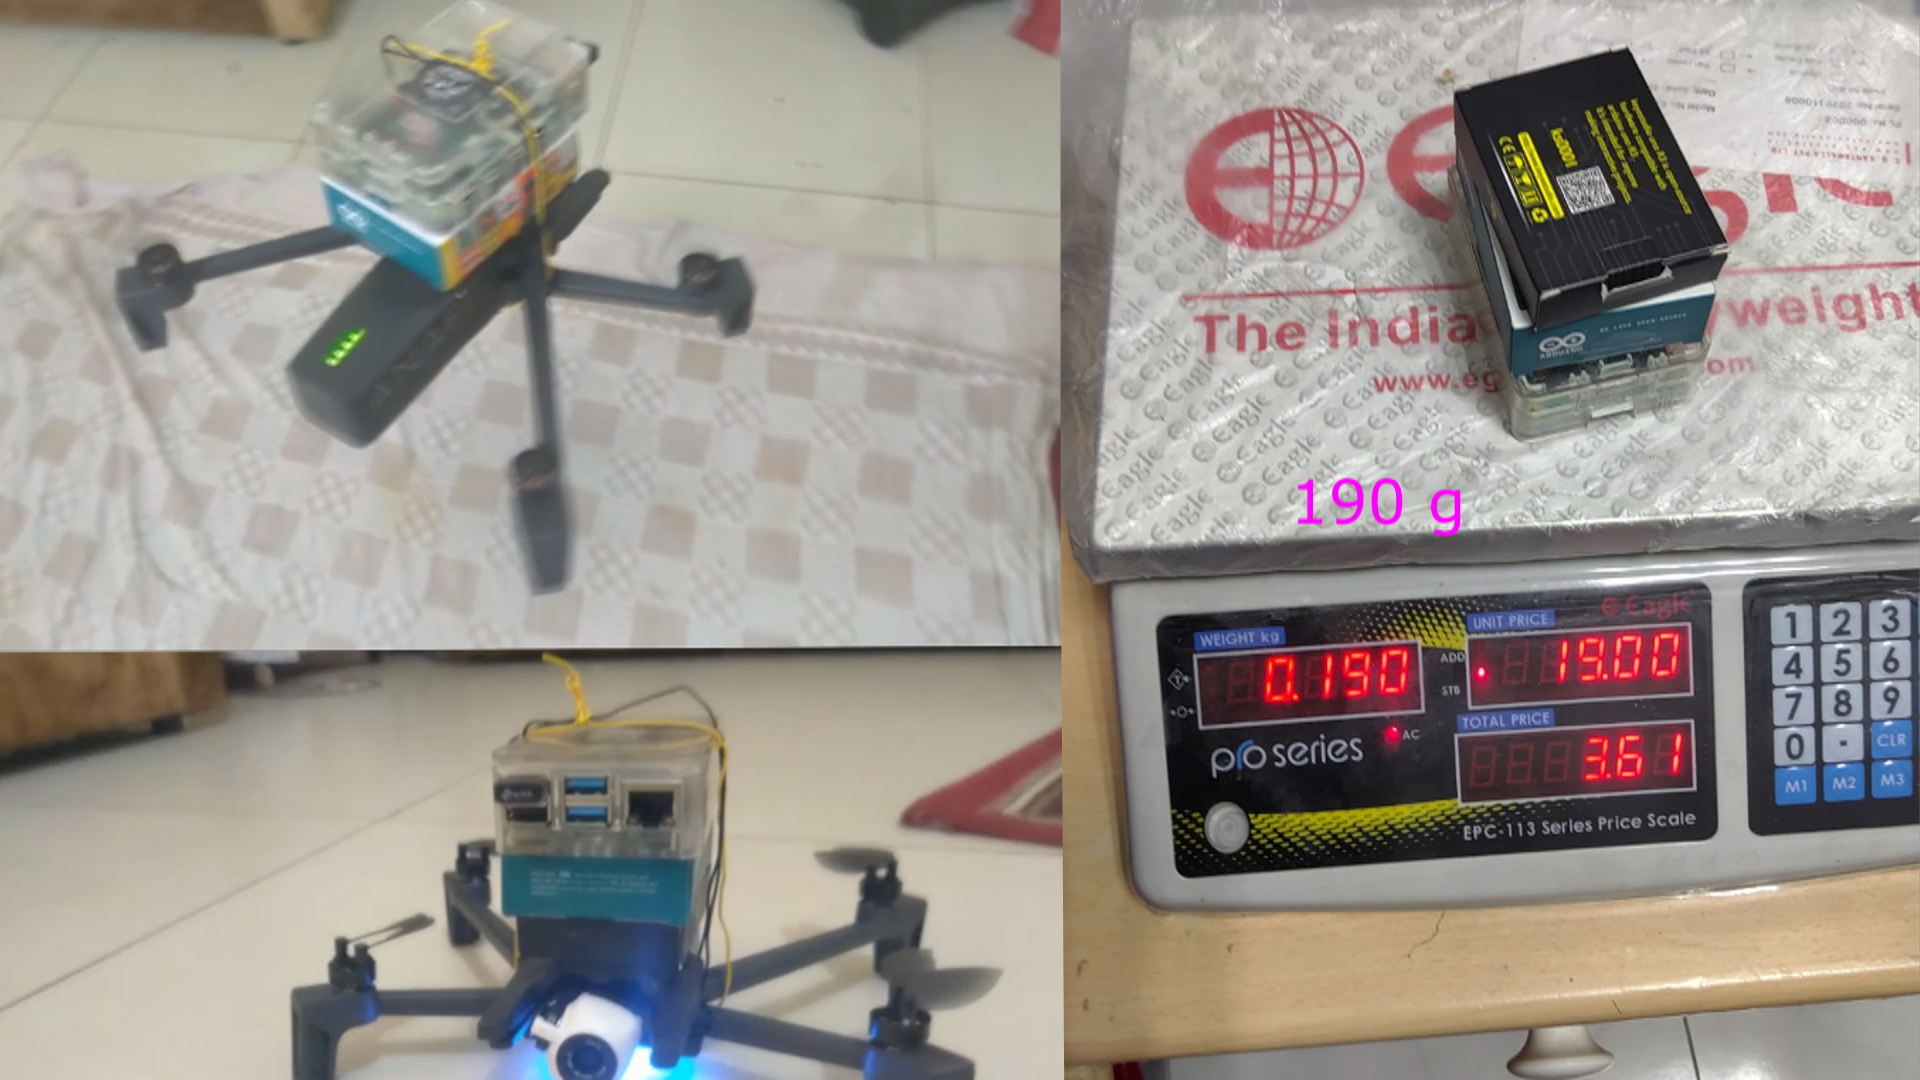
\includegraphics[width=0.6\textwidth]{payload.png}
	\caption{The total weight of the payload}
	\label{fig:payload}
\end{figure} 



% SOFTWARE
\subsection{Simulating the targets}

\lipsum[1]

\subsection{RL training}

\lipsum[1]

\subsection{RL model performance}

\lipsum[1]

\subsection{User interface}

\lipsum[1]


\end{document}
